% -*-latex-*-
% Document name: controls.tex
% Creator: Rob MacLeod [macleod@vissgi.cvrti.utah.edu]
% Last update: September 2, 2000 by Rob MacLeod
%    - created
% Last update: Sun Sep 24 22:21:49 2000 by Rob MacLeod
%    -  Version 5.0Beta release edition
% Last update: Mon Jul 23 13:28:30 2001 by Rob MacLeod
%    - release 5.2
% Last update: Fri Mar 1 20:00:00 2002 by Bryan Worthen
%    - release 5.3
% Last update: Fri Jan 24 20:00:00 2003 by Bryan Worthen
%    - release 5.3
% Last update: Fri Apr 2  20:00:00 2004 by Bryan Worthen
%    - release 6.0
% Last update: Wed Jun 30 13:28:30 2004 by Bryan Worthen
%    - release 6.1
% Last update: Fri Aug 26 13:28:30 2005 by Bryan Worthen
%    - release 6.4
% Last update: Fri Feb 16 09:17:08 2007 by Rob Macleod
%    - version 6.5
%%%%%%%%%%%%%%%%%%%%%%%%%%%%%%%%%%%%%%%%%%%%%%%%%%%%%%%%%%%%%%%%%%%%%%
%%%%%%%%%%  Figures used in this file %%%%%%%%%%%%%%%%%%%%%%%%%%%%%%%%
%begin{latexonly}
  \graphicspath{ {figures/} }
  \newcommand{\mouseaction}%
  {\centerline{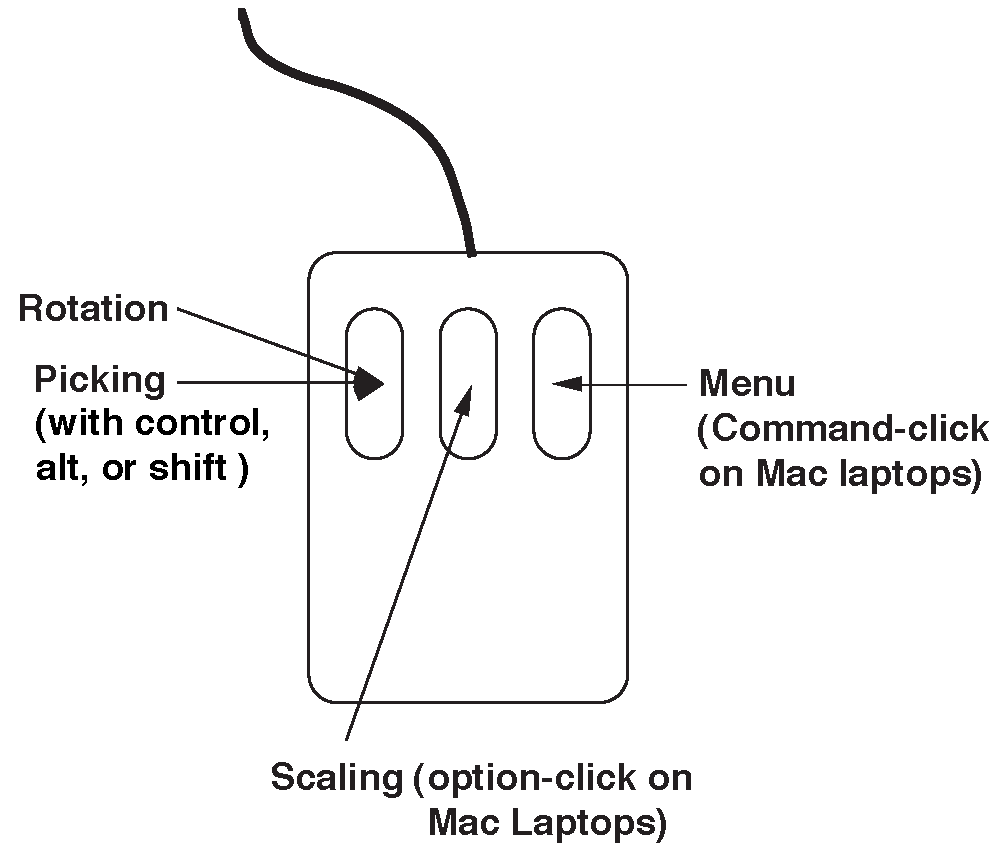
\includegraphics[height=2in]{mouse.pdf}}}
  \newcommand{\filesdialogone}%
  {\centerline{\includegraphics[width=\columnwidth]{filesdialog1}}}
  \newcommand{\filesdialogthree}%
  {\centerline{\includegraphics[width=\columnwidth]{filesdialog3}}}
  \newcommand{\savedialog}%
  {\centerline{\includegraphics[scale=0.75]{savedialog}}}
  \newcommand{\fiducialswindow}%
  {\centerline{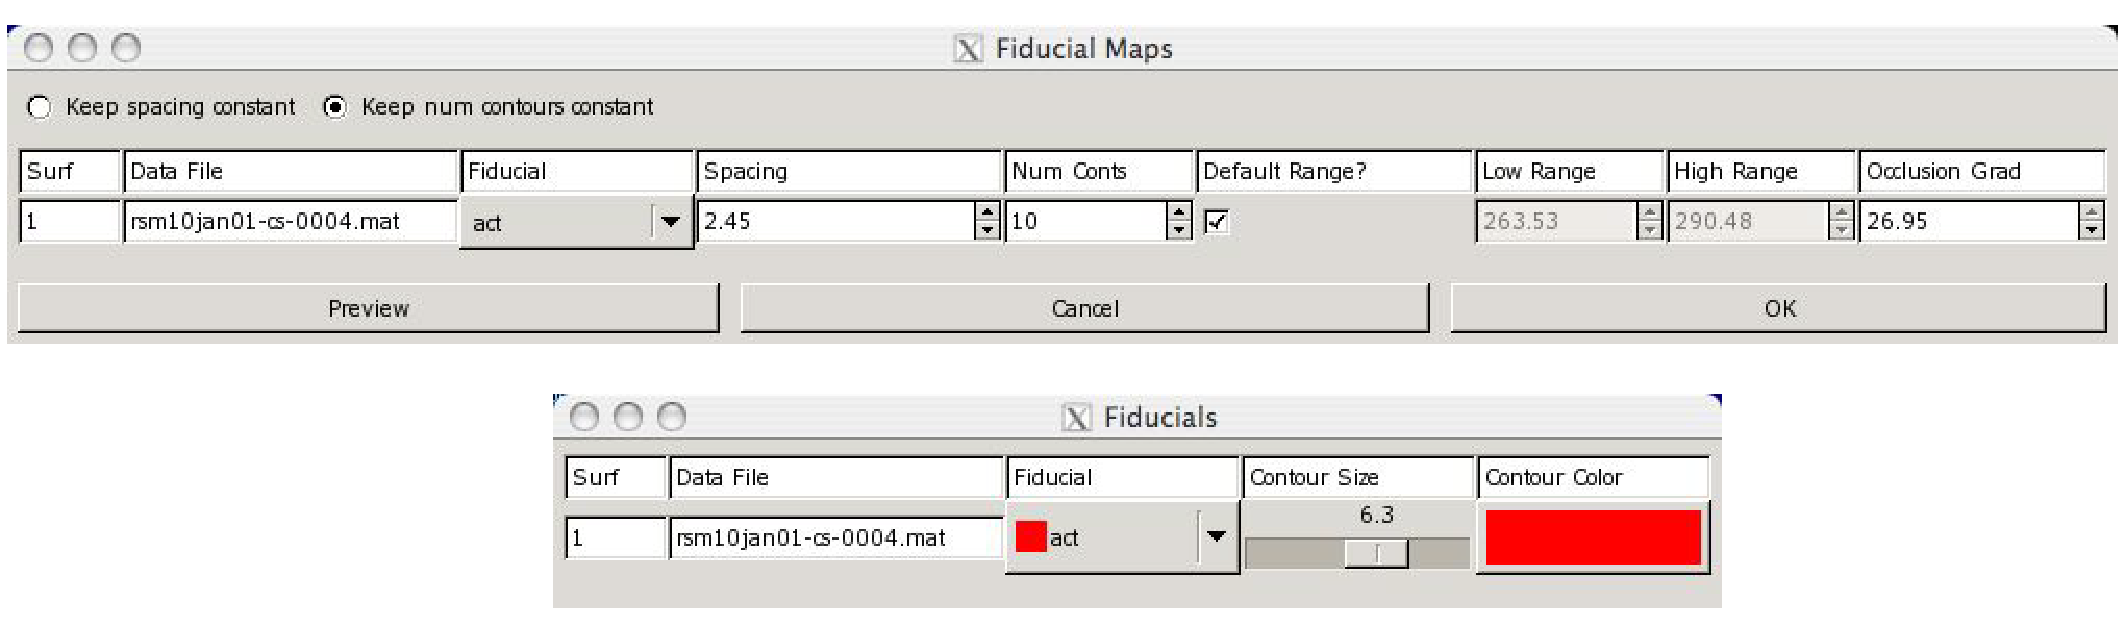
\includegraphics[width=\columnwidth]{fidwindows}}} 
  \newcommand{\fidexamples}%
  {\centerline{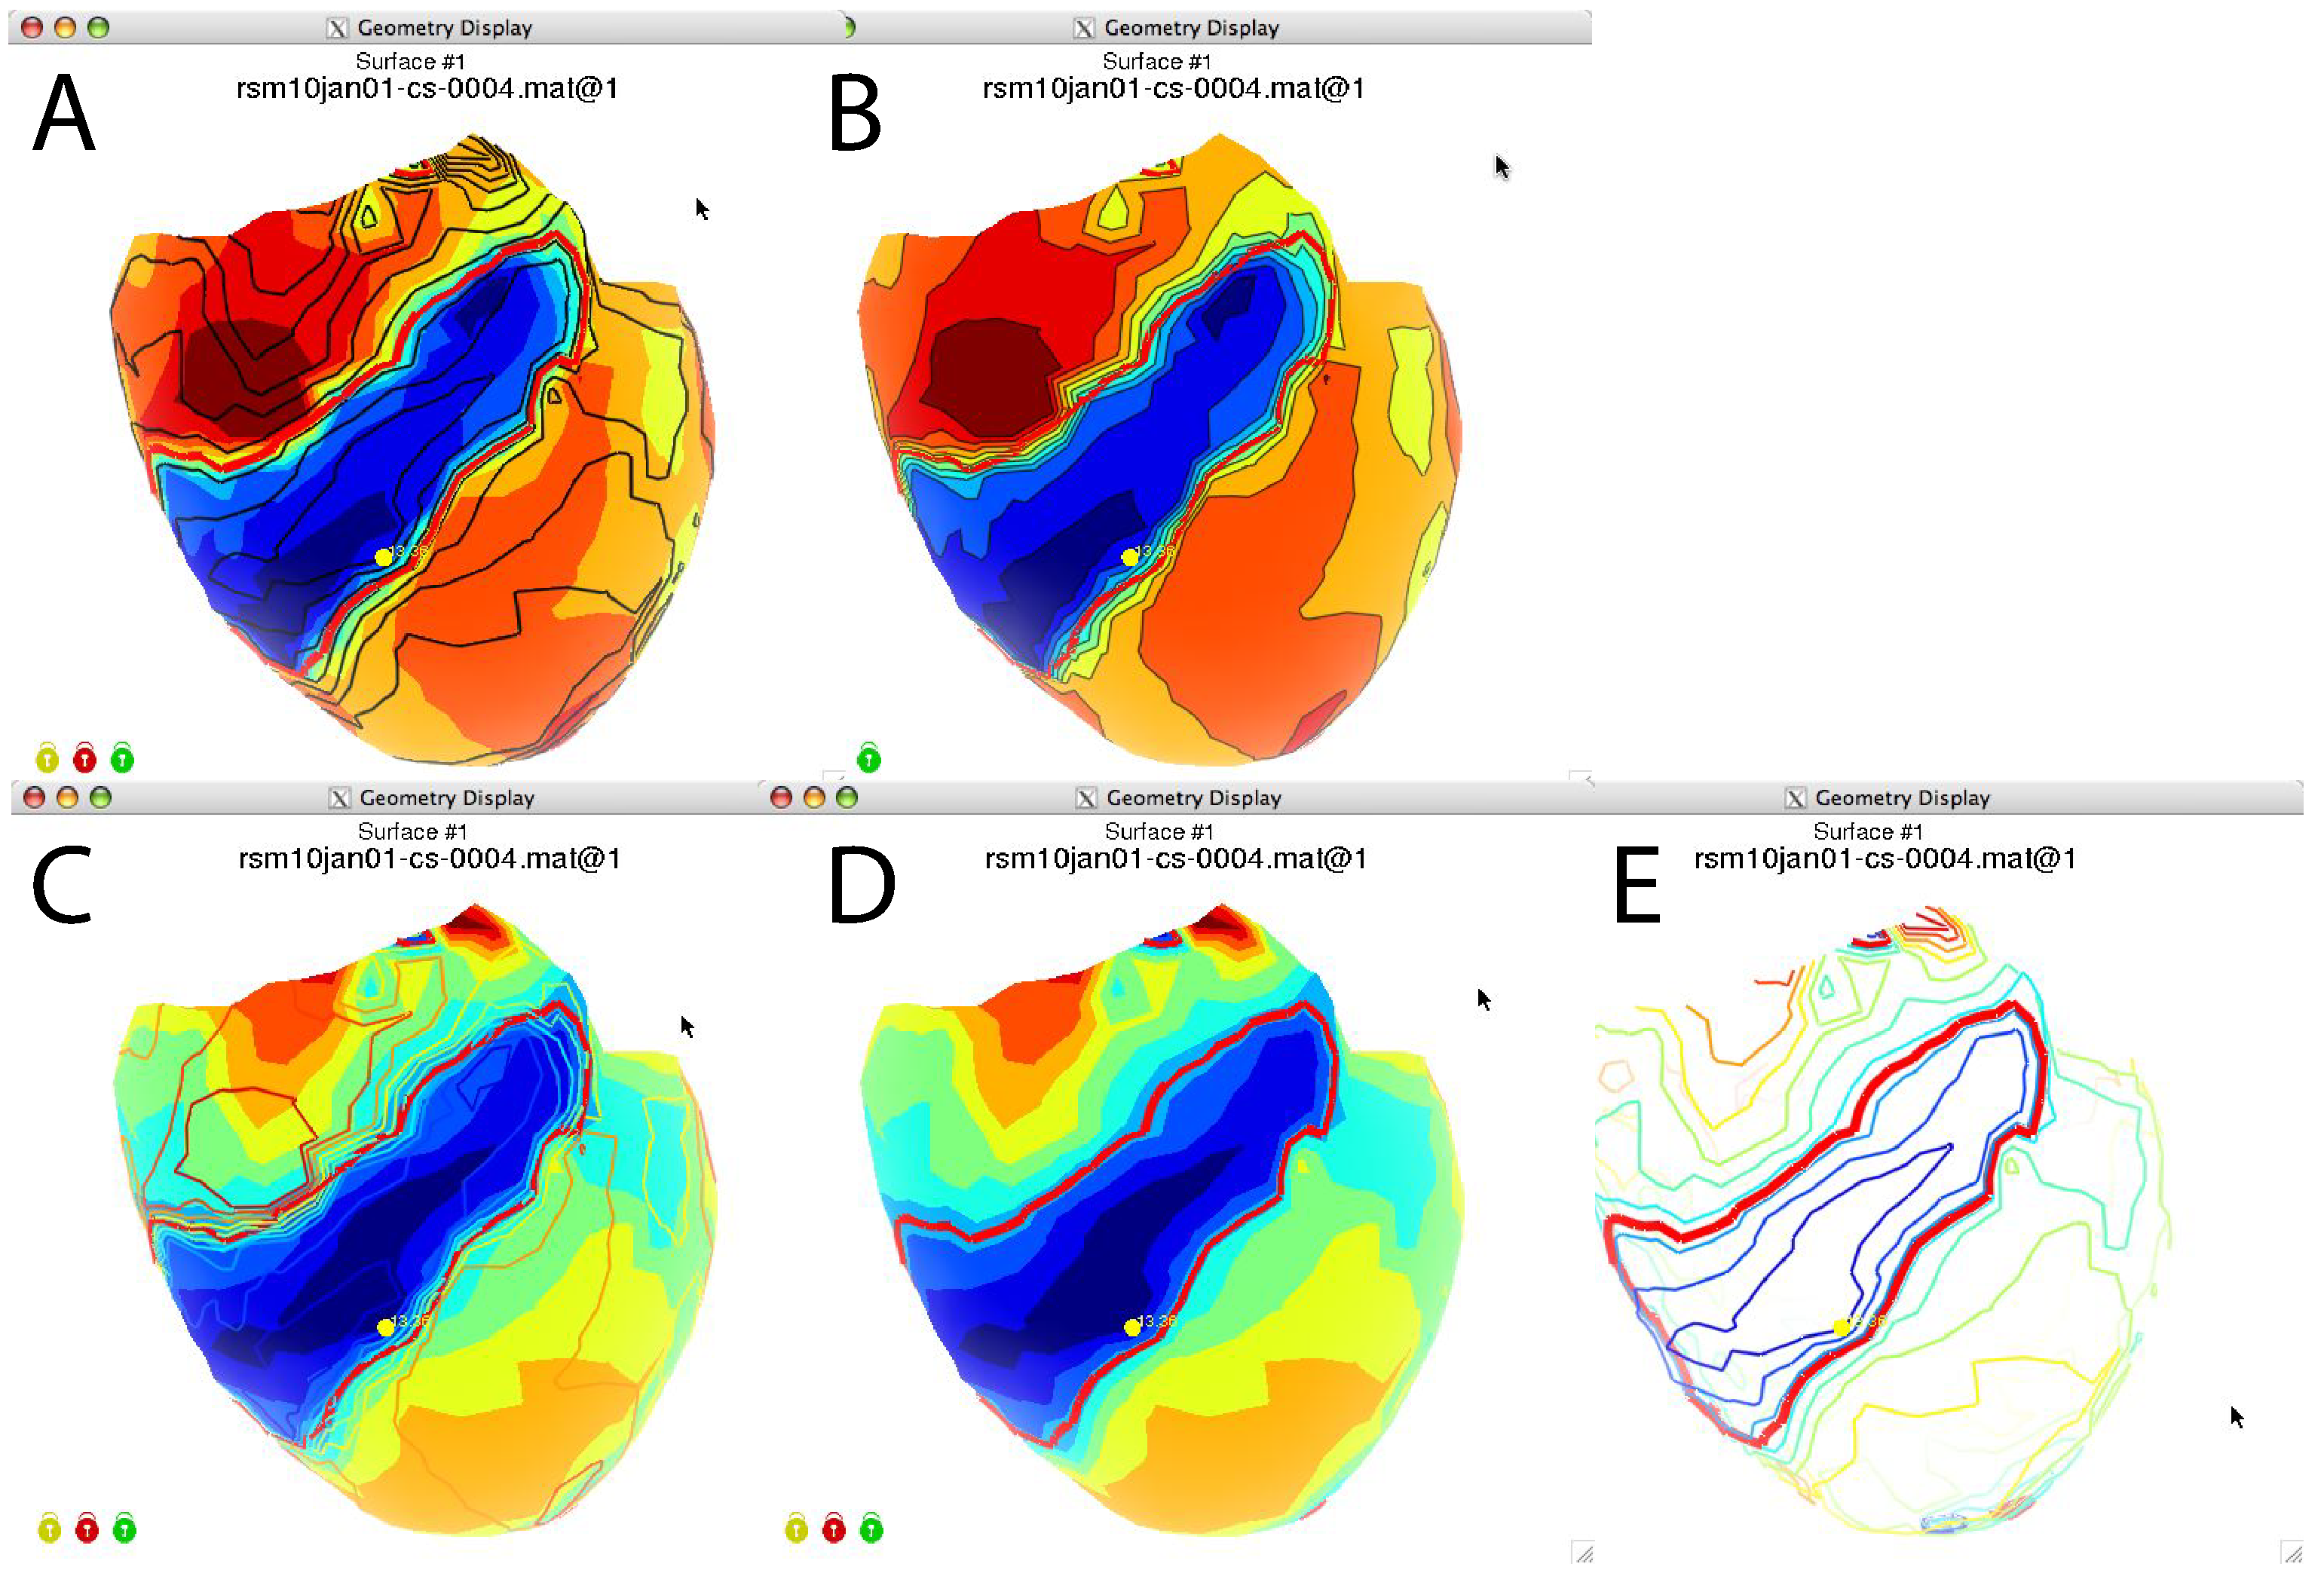
\includegraphics[width=\columnwidth]{fidexamples}}} 
  \newcommand{\scaledialog}%
  {\centerline{\includegraphics[height=2.5in]{scaledialog}}}
  \newcommand{\contourdialog}%
  {\centerline{\includegraphics[height=2.5in]{contourdialog}}}
  \newcommand{\colorpicker}%
  {\centerline{\includegraphics[height=1in]{colorpicker}}}
  \newcommand{\sizepicker}%
  {\centerline{\includegraphics[height=1in]{sizepicker}}}
%end{latexonly}
\begin{htmlonly}
  \graphicspath{ {../figures/} }
  \newcommand{\mouseaction}{%
  \htmladdimg[align=top,width=371,alt="mouse action"]
  {mouse.jpg}}
  \newcommand{\filesdialogone}{%
  \htmladdimg[align=top,width=600,alt="Files Dialog"]
  {filesdialog1}}
  \newcommand{\filesdialogthree}{%
  \htmladdimg[align=top,width=605,alt="Empty Files Dialog"]
  {filesdialog3}}
  \newcommand{\savedialog}{%
  \htmladdimg[align=top,width=415,alt="Save Dialog"]
  {savedialog}}
  \newcommand{\fiducialswindow}{%
  \htmladdimg[align=top,alt="Fiducials Window"]
  {fidwindows}}
  \newcommand{\fidexamples}{%
  \htmladdimg[align=top,width=731,alt="Fiducial Display Examples"]
  {fidexamples.jpg}}
  \newcommand{\scaledialog}{%
  \htmladdimg[align=top,width=791,alt="Scaling Dialog"]
  {scaledialog}}
  \newcommand{\contourdialog}{%
  \htmladdimg[align=top,width=717,alt="Contour Dialog"]
  {contourdialog}}
  \newcommand{\colorpicker}{%
  \htmladdimg[align=top,width=568,alt="Color Picker"]
  {colorpicker}}
  \newcommand{\sizepicker}{%
  \htmladdimg[align=top,width=532,alt="Size Picker"]
  {sizepicker}}
\end{htmlonly}
%%%%%%%%%%%%%%%%%%%%%%%%%%%%%%%%%%%%%%%%%%%%%%%%%%%%%%%%%%%%%%%%%%%%%%
\newpage
\section{Control of \map{}}
\label{sec:control}

This section describes all the means of controlling the function of \map{},
at least all the ones we are willing to tell you about.


%%%%%%%%%%%%%%%%%%%%%%%%%%%%%%%%%%%%%%%%%%%%%%%%%%%%%%%%%%%%%%%%%%%%%%

\subsection{Control by surface}

There is an ever growing number of parameters that the user can alter
for displaying the surfaces in \map{}.  Some of the more important (and
stable) include the following:

\begin{description}
  \item [Visibility:] of points, mesh, potentials, vectors, \etc{} can all
        be controlled individually by using the appropriate function key
        (see Section~\ref{sec:control-keys}), 
      \item [Lead markings: ] of the nodes in the geometry according to
        their node number, channel number, lead number or even value,
  \item [Landmarks: ] appearance of the landmarks on the surface.
\end{description}

Since this level of control is provided for each surface, it is possible to
have points showing on one surface, mesh on another, and rendered potential
shading on a third, and so on. 

\subsubsection{Selecting which surface to control} 
\label{sec:locks} 

To control the display of each surface, be that a surface in its own window
or sharing a single window with other surfaces, a user must select that
surface.  Otherwise, display options will affect all the surfaces.  There
are two different multi-surface situations and each has its own method of
selecting the surface:
%
\begin{center}
  \begin{tabular}{|l|p{3in}|}\hline
    \multicolumn{2}{|c|}{Selecting surfaces for display controls} \\ \hline
    \multicolumn{1}{|c|}{Multi-surface layout} & 
    \multicolumn{1}{c|}{Selection method} \\ \hline
    One surface per window & Mouse location establishes currently active
    window. \\
    Several surfaces in one window & Up/down arrows selects the surface.
    Hitting 
    the up-arrow key after selecting the last surface selects all surface. \\
    \hline 
  \end{tabular}
\end{center}

Note that in the surface window, the lock icons in the lower left corner
indicate if parameter settings act on all surface (locks visible) or just
single surfaces (locks invisible).  Each lock controls a different aspect of 
\map{}:

\begin{description}
  \item [General Lock:] is represented by the yellow (or first) lock icon.  
        When this lock is active, menu items and keyboard commands pertain 
        to all surfaces.  To turn this lock off and on use the up
        and down arrow keys.
  \item [Transformation Lock: ] is represented by the red (or second) 
        lock icon.  When this lock is active, rotation and translation 
        pertain to all surfaces. To turn this lock on and off, use the
        ``t'' key.
  \item [Frame Lock: ] is represented by the blue (or third) lock icon.
        When this lock is active, frame advancing, retreating, and resetting
        pertain to all surfaces.  To turn this lock on and off, use the
        ``f'' key or select from the menu under \emph{Frame Controls}.
\end{description}

Note: in the case where all surfaces are in the same window, unlocking the
general lock by means of the up or down arrow keys selects the single
surface to display.  However, when the general lock is active and either of
the other locks is disabled, the active surface mesh appears in a different
color (blue by default).  This identifies the selected surface and all
modifications apply to this surface.  To select the desired surface use the
(/) keys; ``('' selects the next surface and ``)'' selects the previous.



%%%%%%%%%%%%%%%%%%%%%%%%%%%%%%%%%%%%%%%%%%%%%%%%%%%%%%%%%%%%%%%%%%%%%%

\subsection{Mouse control, keyboard mapping, dials, and menus}
 
Direct interactive control of \map{} is by the keyboard and mouse.
%mouse, and dials.
Many option are available via the menus controlled with the right mouse
button, while others can be activated or toggled with single keystrokes.
Variable (non-binary) adjustments usually occur 
% with the dials, if they are present, 
through dialogues, or by repeating keystrokes.  Below are tables of all the
current control devices and their function.  When the program launches, the
user sets one or more windows which can be resized and moved at any time.
When launching the program with the {\tt -b} option, the resulting
borderless sub-window(s) can still be moved and resized within a main
window using the Alt-key together with the left and middle mouse buttons
respectively.  In Mac OS X and other operating systems where the Alt-key is
mapped to another function you may use the CRTL+SHIFT keys as an
alternative to the Alt-key.


\subsubsection{Mouse control}
\label{sec:control-mouse} 

The mouse can be used for different purposes. Figure~\ref{fig:mouse} 
shows the various actions of the mouse
buttons. 

\begin{figure}[htb]
  \begin{makeimage}
  \end{makeimage}
  \mouseaction
  \caption{\label{fig:mouse} Mouse action for \map{}. Picking
  makes intensive use of the mouse, as does moving objects in the surface
  window.}
\end{figure}

\paragraph{In surface windows: } when the mouse is over a surface window,
mouse buttons have the following actions:
\begin{center}
  \begin{tabular}{|l|l|p{3in}|} \hline
    \multicolumn{3}{|c|}{Mouse Actions}\\ \hline
    \multicolumn{1}{|c|}{Control Key} & 
    \multicolumn{1}{|c|}{Button} & 
    \multicolumn{1}{|c|}{Action}\\ \hline
    None & Left & rotation objects \\
    & Middle & scale objects (downwards increases size, upwards decreases
    size) \\ 
    & Right & activate pull-down menu \\ \hline
    Cntrl & Left & pick a node (and if time series data is present, select the
    channel to display in the time series window) \\
    & Middle &  no action \\
    & Right &  no action \\ \hline
    Shift & Left & translate objects \\
    & Middle & scale objects (rotates clipping planes if they are active
    - more info later) \\ 
    & Right & no action \\ \hline
\end{tabular}
\end{center}

\paragraph{In borderless windows: } when the mouse is over a 
surface within a borderless main window (-b option), the buttons have the
following additional actions: 
\begin{center}
  \begin{tabular}{|l|l|p{3in}|} \hline
    \multicolumn{3}{|c|}{Mouse Actions}\\ \hline
    \multicolumn{1}{|c|}{Control Key} & 
    \multicolumn{1}{|c|}{Button} & 
    \multicolumn{1}{|c|}{Action}\\ \hline
    Alt(Ctrl+Shift)   & Left & Move a single surface subwindow \\ 
      & Middle & Resize single surface subwindow (no indication of change
    until release of mouse button).\\ 
      & Right & no action \\ \hline
  \end{tabular}
\end{center}

Note: if \map{} does not respond as described in these tables, it may be
that your window manager is grabbing the mouse/key combinations for its own
purpose or maps the keys a little differently.  This will require some
setting changes for the window manager.  In Linux there is usually a
control panel or utility application to manage all window system
interactions.

%\newpage

\subsubsection{Keyboard controls}
\label{sec:control-keys} 

Each key of the regular keyboard, the function keys, and the keypad may be
mapped to some function of the \map{}.  Some keyboard keys serve as toggles
to change between a mode being on or off, \eg{} ``n'' toggles the display
of node markings.  Others cycle through a set of choices, \eg{} ``m'' runs
through a series of display options for the mesh.  Several lists of the
keyboard keys and their functions are shown in
Tables~\ref{table:keys}--\ref{table:keypad}.

\begin{table}[htbp]
%\nopagebreak[4]
        \caption{\label{table:keys} Keyboard controls for Geometry Window
          in map{}.  When control contains both lower and upper cases of a
          letter, one cycles through a parameter in one direction and the
          other in the reverse direction.}
    \begin{center}
        \begin{tabular}{|l|p{6in}|} \hline
        \multicolumn{2}{|c|}{\textbf{Regular keyboard}} \\ \hline
        a/A-key   &       Switch colour tables \\ \hline
%        B-key  &       Toggle clipping plane \\ \hline
        c-key   &       Toggle contour draw  (also, when fiducial display
	is active, toggles betwen fiducial contours and scalar data contours \\ \hline
        d-key   &       Toggle depth cuing\\ \hline
%        E-key   &       Toggle back-facing visibility\\ \hline
        f-key   &       Toggle frame lock (also in Time signal window)\\ \hline
%        F-key   &       Shift focus to next window \\ \hline
       g-key   &       Toggle style of Gouraud shading (between
       texture-mapped and non-texture-mapped) \\ \hline 
%       H-key   &       Set the location of the video box \\ \hline
        i-key   &       Toggle ``direction'' (invert) of color table\\ \hline
        l-key   &       Toggle use of lighting\\ \hline
        m/M-key   &       Step through mesh/node drawing options \\ \hline
        n-key   &       Toggle display of node labels (some node marking
        must be selected)\\ \hline 
%        O-key   &       Toggle ortho/perspective views \\ \hline
        p-key   &       Toggles whether surface shading affects scalar data map or
	fiducial map \\ \hline 
         q-key   &       Quit or destroy a sub-window - Legend Window and
         Time Signal Window only (Escape quits the 
                         whole program) \\ \hline
        r-key   &       Reset to startup conditions \\ \hline
        R-key   &       Reset shading model (to wireframe rendering) \\ \hline
%       S-key   &       Saves a .pts and a .fac file of the current 
%       geometry \\ \hline
        s/S-key   &      Cycle through the various surface data draw 
        options (affecting either the scalar data map or the fiducial map - see p-key)\\ \hline
        t-key   &       Toggle transformation lock \\ \hline
%        T-key   &       Whatever Rob is currently testing \\ \hline
%       U-key   &       Toggle locking of clipping planes \\ \hline
%       V-key   &       Toggle video mode \\ \hline
        w-key   &       Write an image to a file.  This will append a 4-digit 
                        number representing a image sequence number to the 
                        base filename (before the extension).  The base 
                        filename can be set at start-time with the -if flag 
                        (see Section~\ref{sec:usage-global}), or in the 
                        Image/Animation Control Dialog (Section~\ref{sec:saving}).  \\ \hline
        x-key   &       Draw axis \\ \hline
%        Z-key   &       Rotate about z-axis in steps \\ \hline
        Escape  &       Quit the program, if pressed in a Geometry Window, 
            or Destroys a Time Signal Window if pressed there. \\ \hline
        +/- key   &    Increases/Decreases size of of currently-selected object
       (see Section~\ref{sec:interactive-size})\\ \hline
       ( \& ) keys   &  Change which surface inside a window will be affected
            when the general lock is on but the transform or frame lock is off
            (see Section~\ref{sec:locks})\\ \hline
\end{tabular}
\end{center}

\end{table} 

\begin{table}[htbp]
%\nopagebreak[4]
        \caption{\label{table:clipping} Clipping plane controls}
    \begin{center}
        \begin{tabular}{|l|p{6in}|} \hline
        \multicolumn{2}{|c|}{Clipping Controls} \\ \hline
        \verb|<|-key    &       Toggle front clipping plane \\ \hline
        \verb|>|-key   &       Toggle rear clipping plane \\ \hline
        [ \& ] keys   &     Move front clipping plane in (initially) +z/-z
             direction respectively \\ \hline
        \{ \& \} keys   &   Move rear clipping plane in (initially) +z/-z
                  direction respectively \\ \hline
        ,-key   &  Lock/Unlock clipping plane rotation with object
                   rotation (when unlocked, shift-Middle-click rotates clipping
                   planes) \\ \hline
        .-key   &  Lock/Unlock clipping planes from each other.
                   When active, clipping planes move together \\ \hline
\end{tabular}
\end{center}

\end{table} 

\begin{table}[htbp]
    \caption{\label{table:arrowkeys} Control of \map{} via the arrow keys}
\begin{center}
    \begin{tabular}{|l|l|} \hline
        \multicolumn{2}{|c||}{\textbf{Arrow Keys}} \\ \hline
        Left Arrow Key  &       Retreat by current frame step (Also in Time
        Signal Window) \\ 
        Right Arrow Key &       Advance by current frame step (Also in Time
        Signal Window)\\ 
        Up Arrow key    &       Select next surface \\
        Down Arrow Key  &       Select previous surface \\ \hline
    \end{tabular}
\end{center}

\end{table}


  %\medskip
\begin{table}[htbp]
    \caption{\label{table:keypad}
      Keypad controls in \map{} - have NUM-Lock off for these to work
      properly.  Again, based on how you have your keys mapped, you might
      have to use the non-keypad keys, but something should work for you
      for each key.}
\begin{center}

\begin{tabular}{|l|p{3in}|} \hline
        \multicolumn{2}{|c||}{\textbf{Keypad Keys}} \\ \hline
   Ctrl-Keypad Left-arrow  &  Y-axis rotate, CW (left)  \\ \hline
   Ctrl-Keypad Right-arrow  &  Y-axis rotate, CCW (right)\\ \hline
   Ctrl-Keypad Up-arrow  &  X-axis rotate, CCW (down) \\ \hline
   Ctrl-Keypad Down-arrow  &  X-axis rotate, CW (up) \\ \hline
   Ctrl-Keypad Home  &  Z-axis rotate, CCW  \\ \hline
   Ctrl-Keypad PgUp  &  Z-axis rotate, CW  \\ \hline
   Ctrl-Keypad End  &  Zoom down  \\ \hline
   Ctrl-Keypad PgDn  &  Zoom up  \\ \hline
%        Keypad 0  &  Shift clip plane  & 
%        Keypad .  &  Shift clip plane  \\ \hline
    Alt(or CRTL+SHIFT)-Keypad Left-Arrow  &  -X-translation (left) \\ \hline 
    Alt(or CRTL+SHIFT)-Keypad Right-Arrow  &  +X-translation (right)\\ \hline
    Alt(or CRTL+SHIFT)-Keypad Down-Arrow  &  -Y-translation (down) \\ \hline
    Alt(or CRTL+SHIFT)-Keypad Up-Arrow  &  +Y-translation (up) \\ \hline
    Alt(or CRTL+SHIFT)-Keypad Home  &  -Z-translation (away) \\ \hline
    Alt(or CRTL+SHIFT)-Keypad PgUp  &  +Z-translation (towards)  \\ \hline
        Plus/Minus key  & Increase/Decrease size of
    currently-selected object. (see Section~\ref{sec:interactive-size})\\
\hline
\end{tabular}
\end{center}
\end{table}
\clearpage


\subsubsection{Menu layout}
\label{sec:control-menus}

Access to the menus is by means of the right mouse button, as per the usual
OpenGL convention.  Below is a series of tables of the menu layout for
\map{}'s Geometry Window.

\begin{table}[ht]
\caption{\label{table:menu-geom}
  The overall menu structure in the Geometry Window}.
  \begin{center}
    \begin{tabular}{|l|p{4in}|} \hline
      \multicolumn{2}{|c|}{\textbf{Overview of Geometry Window menus}} \\
      \hline \hline 
      Files & Opens the Files Window (see Section~\ref{sec:fileswindow}) \\
      Save & Various saving options \\
      Contours & number or spacing and display features of the contours \\
      Fiducials & Fiducial display features - Currently only opens the fiducial
        dialog.  (See Section~\ref{sec:fiducialswindow})\\
      Frame Controls & modifying frame controls\\
      Graphics & general display features such as lighting, clipping,
        and depth cuing \\
      Landmarks & features for toggling and displaying landmarks \\ 
      Mesh & display features of the mesh \\
      Node marking & marking of the nodes \\
      Picking & selecting times signals, mesh information, or other direct
      interactions with the display via the mouse\\
      Scaling & links between data values and color\\
      Surface Data & display features of the scalar data displayed on the
      mesh \\  
      Use +/- to select & Select a feature to change interactively with + or -
      \\
      Window Attributes & features of the windows such as color and text
      labels \\ \hline
    \end{tabular}
  \end{center}
\end{table}

\begin{table}[ht]
\caption{\label{table:saving}Menus for saving options.}
  \begin{center}
    \begin{tabular}{|l|l|p{3 in}|} \hline
      \multicolumn{3}{|c|}{\textbf{Save Menu}} \\ \hline
    Image/Animations & &  Opens the Save Window (see Section~\ref{sec:saving})  \\
    Settings & & Saves a .map3drc file from the currently used settings. This
        file goes in your home directory nad loads each time you run \map{}, so
	it will behave similarly each time. \\
    Script file & & Saves a script file (bash) that loads all the files and
        applies all the settings to recreate the current view (see Section~\ref{sec:scripts}) \\
    Windows batch file & & Saves a windows batch file that loads all the files
        and applies all the settings to recreate the current view (see Section~\ref{sec:scripts})\\ \hline
    \end{tabular}
  \end{center}
\end{table}

\begin{table}[ht]
\caption{\label{table:contours}Menus for contour spacing/number.}
  \begin{center}
    \begin{tabular}{|l|l|p{3 in}|} \hline
      \multicolumn{3}{|c|}{\textbf{Contour Menus}} \\ \hline
    Set Contour Num/Spacing & & Opens a dialog to change user-specified 
    spacing or number of contours. See Section~\ref{sec:contourwindow}.
    \\ 
    Draw style & & \\
    & Dashed line for negative values & draw positive contours in solid,
    negative in broken lines\\
    & Solid lines for all contours & draw all contours in solid lines\\
    Line size & & set the line thickness \\ \hline
    Toggle contours & & toggle display of contours
    without changing settings \\ \hline
    \end{tabular}
  \end{center}
\end{table}

\begin{table}[ht]
\caption{Frame Controls.}
  \begin{center}
    \begin{tabular}{|l|l|p{2.8 in}|} \hline
      \multicolumn{3}{|c|}{\textbf{Frame Control Menus}} \\ \hline
    Lock Frames  & & toggle whether frames 
        operations affect one surface or all surfaces \\ \hline
    Set Frame Interval & & \\
      & Set Frame Step & Opens a dialog to interactively set User-specified 
    frame step.  Affected surfaces are determined by the lock status.\\
      & User-specified Interval & use the value of interval specified in the 
        \texttt{-i} option of the command line or the value set in the
        frame step dialog.\\ 
      & \emph{value} & select between 1 and 90 for frame animation step \\
    Reset Frames to 0 & & positions the surface at the first position in time
       \\
    Align meshes to this frame num & & Positions all surfaces' frames to the
    current surface.  What 'current surface' means will vary based on the status
    of the locks (see Section~\ref{sec:locks})
    \\
    Set time to zero & & Set current frame to be time zero.
        \\ \hline
    Frame Looping & & Allows keyboard frame navigation to cycle around when it reaches the end.
        \\ 
    \end{tabular}
  \end{center}
\end{table}

\begin{table}[ht]
\caption{Graphics menus.  These control general graphic rendering options.}
  \begin{center}
    \begin{tabular}{|l|l|p{3 in}|} \hline
      \multicolumn{3}{|c|}{\textbf{Graphics Menus}} \\ \hline
    Light source & & select the source for the lighting model\\
    & From above &  \\
    & From below &  \\
    & From left &  \\
    & From right &  \\
    & From front &  \\
    & From back &  \\
    & None & no lighting (turn lighting off) \\ \hline
    Toggle clipping & & toggles particular clipping plane options \\
    & Front plane & toggles front clipping plane \\
    & Back plane & toggles rear clipping plane \\
    & Locking planes together & makes planes translate together\\
    & Locking planes with object & rotate surface with the planes or
        rotate surface through the planes \\
    Toggle Depth cue & & apply/disable depth cuing (fog) \\
    Adjust Depth cue & & Opens a dialog to adjust the front and rear planes
    to where the depth cuing occurs. \\
    \hline
    \end{tabular}
  \end{center}
\end{table}

\begin{table}[ht]
\caption{Submenus for the Mesh Display menu}
  \begin{center}
    \begin{tabular}{|p{1in}|p{2in}|p{2.5in}|} \hline
      \multicolumn{3}{|c|}{\textbf{Mesh render menu}} \\ \hline
    Render as & & \\
      &  None & Do not render the mesh \\
      &  Elements  & render filled surfaces for all elements \\
      &  Connectivity & render connectivity mesh\\ 
      &  Elements and connectivity & rendered front facing triangles as
            elements and back facing as connectivity \\ 
      &  Points & render points \\ 
      &  Points and connectivity & render both points and connectivity \\ 
      \hline
    Line/point size 
      & \multicolumn{2}{|l|}{set the size of the mesh's points and lines}\\
    \hline 
    Color 
      & \multicolumn{2}{|l|}{set the color of the mesh}\\ \hline
    Secondary Mesh Color
      & \multicolumn{2}{|l|}{set color of active mesh when multiple 
        surfaces are in same window} \\ \hline
    Show Legend Window
      & \multicolumn{2}{|l|}{display mesh's legend window}\\ \hline
    Hide Legend Window
      & \multicolumn{2}{|l|}{turn off display of mesh's legend window}\\ \hline
    Reload Geometry
      & \multicolumn{2}{|l|}{reload file associated with this geometry}\\
    \hline 
    Reload Surface Data
      & \multicolumn{2}{|l|}{reload file associated with this geometry's
    surface data}\\ \hline 
    Reload Both Geometry and Data
      & \multicolumn{2}{|l|}{reload files associated with this geometry and
    its data}\\ \hline 

    \end{tabular}
  \end{center}
\end{table}

\begin{table}[ht]
    \caption{\label{table:nodemarking} Menus for marking nodes in the display.
      If all surfaces are currently displayed, any of these settings will affect
      all surfaces based on the rules in locks section (see
      Section~\ref{sec:interactive-size}).  If we have a single  
      or current) surface only, then change only that surface.}
  \begin{center}
    \begin{tabular}{|l|l|p{4 in}|} \hline
      \multicolumn{3}{|c|}{\textbf{Node Marking Menus}} \\ \hline
    All & & Make all the nodes in this (or all) surface(s) \\
    &  Sphere & mark each node with a sphere \\
    &  Map data to spheres & mark each node with a sphere, whose
                             color reflects its scalar data value \\
    &  Node \# & mark each node with the node number in the geometry \\
    &  Channel \# & mark each node with the associated data channel number \\
    &  Data value & mark each node with the associated data value \\
    &  Color & set the color for marking all nodes \\
    &  Size & set the size of all node markings \\
    &  Clear all marks & remove all node marking settings \\ 
    \hline
    Extrema & & Make all the nodes that are the extrema  \\
    &  Sphere & mark each extrema with a sphere \\
    &  Node \# & mark each extrema with the node number in the geometry \\
    &  Channel \# & mark each extrema with the associated data channel
    number \\ 
    &  Data value & mark each extrema with the associated data value \\
    &  Size & set the size of all extrema markings \\
%    &  Color & set the color for marking all extrema \\
    &  Clear all marks & remove all extrema marking settings \\ 
    \hline
    Time signal & & Make all the nodes that identify the location of time
    signals shown in the display  \\
    &  Sphere & mark each times signal location with a sphere \\
    &  Node \# & mark each times signal location with the node number in
    the geometry \\ 
    &  Channel \# & mark each times signal location with the associated
    data channel number \\ 
    &  Data value & mark each times signal location with the associated
    data value \\ 
    &  Color & set the color for marking all times signal locations \\
    &  Size & set the size of all time signal markings \\
   &  Clear all marks & remove all time signal marking settings \\ 
    \hline
    Lead links & & Make all the nodes that identify the features from
    leadlinks file 
       (see Section~\ref{sec:leadfiles}) shown in the display  \\
    &  Sphere & mark each lead location with a sphere \\
    &  Node \# & mark each lead location with the node number in
    the geometry \\ 
    &  Channel \# & mark each lead location with the associated
    data channel number \\ 
    &  Data value & mark each lead location with the associated
    data value \\ 
    &  Lead labels & mark each lead with the label from the leadlinks file.\\
    &  Color & set the color for marking all lead locations \\
    &  Size & set the size of all lead markings \\
   &  Clear all marks & remove all lead marking settings \\ 
    \hline
    \end{tabular}
  \end{center}
\end{table}

\begin{table}[ht]
    \caption{\label{table:pickingone} Pick mode menus, part 1.  Picking is
      based on a 
      mode (selectable in this menu), and is done with CTRL-left mouse button
      unless otherwise specified.}
  \begin{center}
    \begin{tabular}{|l|p{4 in}|} \hline
        \multicolumn{2}{|c|}{\textbf{Picking Menus I}} \\ \hline
        Time Signal (new window mode) & create a new time signal window with
        each pick of a node \\
        Time Signal (refresh window mode) & update the last time signal 
        window with each pick of a node \\
        Display node info mode & Picking will cause certain node information
        to be dumped to the console. \\
        Display triangle info mode & Picking will cause information about
        the triangle you click in to be dumped to the console.
        It may be easier to pick triangles with clipping planes on. \\
        Triangle construction/deletion & Normal picking (ctrl-clicking on nodes)
        will select points to form a triangle (triangulate).  Clicking the first 
        two nodes in this fashion will display the selected nodes, and then a 
        line between the two.  When the third is clicked, a new triangle is 
        displayed and added to the geometry. \\
        & CTRL-middle clicking selects a triangle (and not nodes) to be deleted.
        Again, it may be easier to pick triangles with clipping planes on. \\
        Flip triangle mode & Will change the order of drawing the triangle's
        points.  This will cause front-facing triangles to become back-facing
        and vice-versa.  See Section~\ref{sec:display-mesh}, mesh rendering
        options 
        for information on how to tell which way a triangle is facing. \\
        Edit node mode & Will allow you to pick a point and translate it
        with the keyboard transform controls (see
        Section~\ref{sec:control-keys}, keypad controls) \\
        Edit landmark point mode & Will allow you to pick a landmark point
        and translate it with the keyboard transform controls (see
        Section~\ref{sec:control-keys}, keypad controls) \\
        Delete node mode & Will remove from the geometry any node that you pick
        and any triangles associated with it. \\
        \hline
    \end{tabular}
\end{center}
\end{table}

\begin{table}[ht]
  \caption{\label{table:pickingtwo} Pick mode menus, part 2.  Picking is
    based on a 
    mode (selectable in this menu), and is done with CTRL-left mouse button
    unless otherwise specified.}
  \begin{center}
    \begin{tabular}{|l|p{4 in}|} \hline
      \multicolumn{2}{|c|}{\textbf{Picking Menus II}} \\ \hline
    Reference lead, single value & Causes all values to be measured
    against the node which you pick \\
    Reference lead, mean value & Causes all values to be measured
    against a mean value of all the nodes \\
    Reset Reference & Causes the reference and values to be reset to
    its original value.  You must reset the reference if you want to
    change the reference more than once. \\
    Show Time Signal Window info & Toggles display modes in time series window.
    When there is no info, the graph takes up more room in the window. 
    This is equivalent to pressing 'p' in a geometry window or selecting
    the toggle display mode option of a time series window's menu. \\
    Show all pick windows & Causes all Time Series (Pick) Windows
    associated with this geometry to become visible. \\
    Hide all pick windows & Causes all Time Series (Pick) Windows
    associated with this geometry to become hidden. \\ 
    Size of picking aperture & select the size of the region around the
    mouse 
    pointer that will register a ``hit'' when picking; larger values will
    make it easier to pick an object but also easier to hit multiple
    objects. \\ 
    Size of triangulation node mark & when triangulating, a node
    mark will appear on the node(s) selected.  Adjust that mark's size. 
    \\ \hline
    \end{tabular} 
  \end{center}
\end{table}

\begin{table}[ht]
    \caption{Menu for scaling, the mapping from data value to color for
      rendering. }
\label{table:scaling}
  \begin{center}
    \begin{tabular}{|l|l|p{3 in}|} \hline
      \multicolumn{3}{|c|}{\textbf{Scaling Menus}} \\ \hline
    Scaling... & \multicolumn{2}{|l|}{opens up the scaling dialog.  (see
    Section~\ref{sec:scalinggui})} \\
    Range & & \\
    &  Local  & scale based on the local extrema for each surface and time
       instant \\
    &  Global over all frames in one surface  & scale based on the extrema 
        over the full times series \\ 
    &  Global over all surfaces in one frame & scale based on the extrema over 
        each surface for the local time instant\\
    &  Global over all surfaces and frames & scale based on the extrema
    over all surfaces 
       and all time instants\\
    &  Scaling over groups in one frame & scale based on the extrema over 
        each surface in specified group for the local time instant\\
    &  Scaling over groups in all frames & scale based on the extrema over 
        each surface in a specified group for all time instants\\
    &  Slave Scaling over one frame & scale based on the extrema over 
        each surface's master surface (set with -sl in command line)
        for one time instant\\
    &  Slave Scaling over all frames & scale based on the extrema over 
        each surface's master surface (set with -sl in command line)
        for all time instants\\ \hline

    Function & & \\
    &  Linear & linear mapping between value and color \\ 
    &  Logarithmic & color changes as  $\log({\rm value})$ \\ 
    &  Exponential & color changes as  $\exp({\rm value})$ \\ 
    &  Lab standard & color reflects lab standard \\ 
    &  Lab 13 standard & color reflects lab 13 standard \\ \hline
    Mapping & & \\ 
    &  True & use true extrema \\ 
    &  Symmetric about zero & take largest of absolute values of extrema to
    determine scaling \\
    &  Symmetric about midpoint & scale independently on both sides of the
    midpoint to determine scaling \\
    &  Separate about zero & scale positive and negative portions of the
    scale independently \\ \hline
    Grouping & & \\
    &  Move to group \# & Select a group to place the current surface
    (make sure the general (yellow) lock is off, or all surfaces
    will be placed in that group) \\ \hline
    \end{tabular}
  \end{center}
\end{table}

\begin{table}[ht]
    \caption{Submenus to control the display of scalar data on the mesh.}
  \begin{center}
    \begin{tabular}{|l|l|p{2.5 in}|} \hline
      \multicolumn{3}{|c|}{\textbf{Surface Display Menus}} \\ \hline \hline
    Color & & \\
    &  Rainbow  & use rainbow color map to render scalar values on the mesh\\
    &  Green to red & use green to red color map\\
    &  White to Black & use black and white color map\\ 
    &  Invert & invert the sense of any color map, \eg{} black becomes
        white and white becomes black \\ \hline
    Render style & & \\
    &  None & Turn Shading off \\
    &  Flat & colour each mesh element in a constant
       color according to the mean value of scalar data over the vertices\\
    &  Gouraud & shade each polygon using linear interpolation \\
    &  Banded & draw the regions between contour lines as bands of constant
       color\\  \hline
    \end{tabular}
  \end{center}
\end{table}

\begin{table}[ht]
    \caption{The Use +/- to interactively change sizes menu}
  \begin{center}
    \begin{tabular}{|l|p{4in}|} \hline
      \multicolumn{2}{|c|}{\textbf{+/-  Adjust Menu.}} \\ \hline \hline
      Large Font Size & Change the largest font size (This is the title
    for the Colormap and Geometry windows) \\ 
      Medium Font Size & Change the medium font size (This is all text
    not small or large) \\ 
      Small Font Size & Change the small font size (This is the size for
    the node marks, the axis labels in the Time Signal Window, and the
    Contour Labels in the ColorMap Window) \\ 
      Contour Size & Change the contour width \\
      Line/Point Size & Change the width of Lines/Points in the mesh \\
      Node Marks (all) Size & Change the width of node marks \\
      Node Marks (extrema) Size & \\
      Node Marks (time signal) Size & \\
      Node Marks (leads) Size & \\
      Change in translation & Change how fast the keyboard translation
    happens \\ 
      Change in scaling & Change how fast the keyboard scaling happens \\
      Change in rotation & Change how fast the keyboard rotation happens
      \\ \hline 
    \end{tabular}
  \end{center}
\end{table}



\begin{table}[ht]
  \caption{Controls for the attributes of the \map{} windows.}
  \begin{center}
    \begin{tabular}{|l|l|p{3 in}|} \hline
      \multicolumn{3}{|c|}{\textbf{Window Attributes Menus}} \\ \hline
    Screen info & & select the text written to the screen.  
    Note that screen info 
       disappears when clipping is on.\\
      & Turn screen info on & \\
      & Turn screen info off & \\ 
      & show/hide lock icons & toggle lock display \\ \hline
      & Show Legend Window & Turns on Colormap window \\ 
      & Hide Legend Window & Turns off Colormap window \\ 
    Color & & select window colors with the separate color selector \\
      & Background & select background color for the window \\
      & Foreground & select foreground color for the window \\ \hline
    Size & & select some size options \\
      & \emph{value} & set window to specified resolution \\
    Axes & & select options for axes \\
      & Axes Color & Select axes color \\
      & Axes Placement & select whether axes displayed per window or mesh \\
      & Toggle Axes & turn on/off axes \\ \hline
    Font Size & & Use the Size Picker to adjust the font size \\
      & Small Font Size & Size of node mark text or Colormap window contour 
        ticks \\
      & Medium Font Size & Size of window subtitles or text in Pick Window \\
      & Large Font Size & Size of Window titles \\
    Toggle Transformation Lock & & toggle whether surfaces transform 
        together or independently \\ \hline
    \end{tabular}
  \end{center}
\end{table}


\begin{table}[ht]
\caption{Controls for the attributes of the Time Signal Window.}
  \begin{center}
    \begin{tabular}{|l|p{4in}|} \hline
      \multicolumn{2}{|c|}{\textbf{Time Signal Window Controls}}
      \\ \hline \hline
      Axes Color & Select Axes Color \\
      Graph Color & Color of data graph \\  
      Toggle Display Mode & Show basic values and graph, show
      detailed values and graph, or show larger
      graph\\ \hline
    \end{tabular}
  \end{center}
\end{table}


\begin{table}[ht]
\caption{Controls for the attributes of the Legend window.}
  \begin{center}
    \begin{tabular}{|l|l|p{3 in}|} \hline
      \multicolumn{3}{|c|}{\textbf{Legend Window Controls}} \\ \hline
    Orientation & & Layout of information in Legend Window\\
      & Vertical & \\
      & Horizontal & \\ \hline
    Number of Tick Marks & & select number of ticks to appear on bar \\
      & 2,4,8 & Either 2,4,8 ticks.  These will not be colored as they do not
        directly correspond to contour values. \\
      & Match Contours & Match number of contours in corresponding geometry
    \\ \hline 
    \end{tabular}
  \end{center}
\end{table}

\begin{table}[ht]
\caption{Controls for the Legend Window Menu}.
  \begin{center}
    \begin{tabular}{|l|p{4in}|} \hline
      \multicolumn{2}{|c|}{\textbf{Main Window Controls}} \\ \hline \hline
      Set Background Color & Select bg Color \\
      Quit Map3D & Quit Map3D \\ \hline
    \end{tabular}
  \end{center}
\end{table}

\clearpage


%  Report level & & \\
%     & \multicolumn{2}{l|}{Level 0 = default} \\
%     & \multicolumn{2}{l|}{Level 1 = report extrema} \\
%     & \multicolumn{2}{l|}{Level 2 = mild debugging}  \\
%     & \multicolumn{2}{l|}{Level 3 = moderate debugging} \\
%     & \multicolumn{2}{l|}{Level 4 = max debugging} \\ \hline
%  \hline
%Save settings & & \\
%   & \multicolumn{2}{l|}{save in local .map3drc} \\
%   & \multicolumn{2}{l|}{save in home .map3drc} \\ \hline

%%%%%%%%%%%%%%%%%%%%%%%%%%%%%%%%%%%%%%%%%%%%%%%%%%%%%%%%%%%%%%%%%%%%%%

%  \subsection{Feedback Reporting Level}

%  In order to control the amount of printed feedback \map{} provides (which
%  is posted in the window from which the program was launched), the user can
%  select a value between 0 and 3 from the a sub-menu of the main menu titled
%  {\em Report level}.  The settings and level of output are as follows:


%  \begin{center}
%  \begin{tabular}{|c|l|} \hline
%    \multicolumn{1}{|c|}{Report Level} &
%    \multicolumn{1}{|c|}{Types of output} \\ \hline
%    0 & minimal output --- just changes in status \\
%    1 & report extrema \\
%    2 & report some warning messages \\
%    3 & debug mode \\ \hline
%  \end{tabular}
%  \end{center}


%%%%%%%%%%%%%%%%%%%%%%%%%%%%%%%%%%%%%%%%%%%%%%%%%%%%%%%%%%%%%%%%%%%%

\subsection{Interactive GUIs - File Selection, File Saving, and Scaling
  Options, \etc{}} 
\label{sec:interactive}

With the move to a dedicated GUI system (in our case, gtk), we make use of
a number of different windows to select parameters and control \map{}.
This section covers the functionality of all of them.

\subsubsection{Files Window}
\label{sec:fileswindow}

\begin{figure}[htb]
  \begin{makeimage}
  \end{makeimage}
  \filesdialogone
  \caption{\label{fig:file1} Files Dialog for \map{}.}
\end{figure}

The most frequently used GUI window is the ``\map{} Files'' window, allows
you to interactively select filenames, data windows, etc.  The others are
for saving files, and for quick scaling changes.  Figure~\ref{fig:file1}
shows an example of such a file window, and access to this window is by
means of the ``Files'' menu option of the main menu.  This window displays
one row for each surface, where each row shows the surface number, the
window the surface appears in, the geometry filename, the geometry number,
the data filename, the start frame number, the end frame number, a graph of
the RMS curve, and a button to show other files.  Most of these columns can
be modified at any time.  If you click on the ``New Surface'' button, an
empty row will pop up, allowing you to add a surface from scratch.
 
None of the changes made to this window will take effect until you click on
the ``Apply'' button.  The  ``Close'' button will cause  the window
will close, but opening it again will reveal the same content.

\begin{table}[htbp]
\caption{\label{table:filewindow} Options for the file window}    
\begin{center}
\begin{tabular}{|l|p{4in}|} \hline
    \multicolumn{2}{|c|}{\textbf{File Window Options}} \\ \hline\hline
    Surf      &      Number of the surface \\ \hline
    Win\#      &      Number of the window that contains this surface.
          You can change this number to move the surface to any
          open window, or to a new window (by selecting the last
          number from the drop-down menu). \\ \hline
    Geom File &      Name of the geometry file of this surface.  To change
        the geom file click on the
        ... button and then browsing for the desired file. You may reload the
        current geometry by  
        selecting the ``Mesh$\Rightarrow$Reload Geometry'' 
        menu entry. \\ \hline
    Geom\#     &      Number of surface within the geometry file (see
         Section~\ref{sec:geomfiles}). 
         If there is more than one surface in the geometry
         file, an associated drop-down  menu selects which one to 
         insert.   \\ \hline
    Geom Save (disk icon) &      Allows saving of the current geometry ( see
         Section~\ref{sec:savegeom}). \\ \hline
    Data File      &   Name of the data file of this surface.
         As with geometry  clicking on the ... button launches 
         a file browser to select a time-series data file.
         Selecting the ``Mesh$\Rightarrow$Reload Data'' reloads
         the data. \\ \hline
    Data Selection &   If more than one time series is present in the data
         file, the selection will allow you to choose between them \\ \hline
    Start Frame           &   Start reading data at this frame. 
         Left-clicking 
         in the graph section and dragging will also  select the
         correct frame. \\ \hline
    End Frame             &       Finish reading data at this frame.
         Middle-clicking in the graph section and dragging 
         will  select the correct frame. \\ \hline 
    Frame Step            &       If larger than 1, \map{} will load every nth frame \\ \hline 
    Graph     &       Graph of the root-mean-square signal calculated
         from all signals in the time series.    Left- or
         middle-clicking in this graph selects the data window that
         \map{} will read and display. \\ \hline 
    Other Files (+)       &       This button will expand another section
         in which to view/modify the channels, leadlinks, 
         landmarks, or fiducial file to use with this surface. \\ \hline 
\end{tabular}
\end{center}
\end{table}


\begin{figure}[htb]
  \begin{makeimage}
  \end{makeimage}
  \filesdialogthree
  \caption{\label{fig:file3} Empty Files Dialog. \map{} will start up this way
            if launched without arguments.}
\end{figure}

Note that the File window allows launching of \map{} without any arguments.
In this case an empty file window appears, as in Figure~\ref{fig:file3} so
that the user can select all the files for display and set up the display
interactively.

\paragraph{Saving Geometry}
\label{sec:savegeom}


When selecting the save icon, a menu will pop up prompting whether \map{}
should save the file with the current transformations or not.
If "Apply transformations" is chosen, then \map{} will save the geometry with the
current transformations (translations and rotations) applied.
Make sure to modify the filename or the current filename will be replaced.  
Files can be named with .mat, .fac, or .pts extensions. If the filename ends
in the extension .fac, it will save filename.fac and filename.pts.
%If Transforms is selected and
%there is a landmarks file, then a filename.lmark.

\subsubsection{Saving Images/Animations}
\label{sec:saving}

\begin{figure}[htb]
  \begin{makeimage}
  \end{makeimage}
  \savedialog
  \caption{\label{fig:save1} Image Control Dialog.}
\end{figure}


\paragraph{Saving Images}
\label{sec:saveimages}

The Image Control dialog is used to control the base filename for saved images
and whether to save animations.  Select a filename (you can click on ... to browse for
a filename) and click save. The filename may have the extension .ppm, ,png,
or .jpg to save in one of those formats.  The final filename also appends a
4-digit number before the extension, representing a number in a sequence of
images.  I.e., if the filename selected is map3d.png, the image will
actually save in map3d0000.png, and subsequent images will be
map3d0001.png, map3d0002.png, etc.  The image that will saved is
approximately the smallest rectangle that contains all open map3d windows.

NOTE: If there are windows that overlap, the one on top might not be the one
\map{} thinks is on top.  So if after moving windows around, it is
necessary to click inside the
window (not the title bar), to tell \map{} it is on the top.  Otherwise,
data that appears on the computer screen may end up obscured by other
windows that appear to lie beneath. 

If the Save... window is in the way, close it, and pressing the 'w'
key will have the same effect as clicking the ``Save Image'' button. 

\paragraph{Saving Animations}
\label{sec:saveanimations}

Checking the "Automatically save image when changes occur" box
allows you to control automatic frame saving to put images 
together into movies.  While \map{} is not yet sophisticated enough to 
actually create the movies, this control can save the images you need and
then you can use some external software to make a movie from them.
See Section~\ref{sec:animation} for links to instructions of how to make 
movies from sets of images. 

\medskip
There are three changes types that determine whether an image will be saved.  
%
\begin{enumerate}
  \item Save Frame on Transformation - will save a frame (image) every
        time you transform (rotate, translate, scale) any surface, either 
        with the mouse or the keyboard.
  \item Save Frame on Frame Advance - will save a frame when you move 
        forward or backward in time with the arrow key, or change the time
        in the pick window.
  \item Save Frame on Other Events - will save a frame when you interact with
        with the Geometry Window in any other way, via keyboard commands or 
        menu controls.
\end{enumerate}
\medskip

Naturally, animations start recording when you check the box, and stop 
when you uncheck the box.

%%%%%%%%%%%%%%%%%%%%%%%%%%%%%%%%%%%%%%%%%%%%%%%%%%%%%%%%%%%%%%%%%%%%%%

\subsection{Controlling the time signal window}
\label{sec:control-scalar} 


There are two ways to create a time signal window:
%
\begin{enumerate}
  \item Specify a \texttt{-at xmin xmin ymin ymax} on the command line
        (optionally with a \texttt{-t trace-lead-number} to specify the
        channel to use).
      \item Using picking (Cntrl-left mouse) to select a lead to show in
        the time signal window, when the current pick mode is time signal
        new-window mode or time signal refresh mode.  Note that subsequent
        time signal picking can be set to either a) update the last time
        signal window to the new data channel or b) add yet another time
        signal window.
\end{enumerate}
%

The format of the scalar display is fairly simple 
%(see Section~\ref{sec:displayscalar})
, with a vertical bar moving along the time axis as the frame number is
advanced.  \map{} derives the time axis label from the frame numbers of the
signal relative to the time series data file, not relative to the subset of
frame read in, \ie{} if frames (or pot file numbers) 10--20 are read in
with an increment of 2, then frame number will begin at 10, and go through
12, 14, 16, 18 and end at 20 rather then beginning at 0 or 1 and going to 10
(the number of frames of data actually read).

%There is also a menu item for adjusting the time base of the signal,
%manually aligning time across multiple windows, and setting the time
%increment between frames of data.

\subsubsection{Adjusting the frame selector}
\label{sec:control-frames} 

In order to facilitate rapid movement through large datasets, the user can
control the frame number being displayed by interacting with the scalar
window itself.  If the user moves the cursor to the scalar window and
pushes the left mouse button, the vertical time bar will jump to the
nearest sample to the cursor location.  The user can then hold the left
button down and slide the time marker left and right and set a desired
frame.  Once the mouse button is released,\map{} updates the map display.
The left and right arrow keys also shift the frame marker back and forth.
The only other command allowed when the cursor is within the scalar window
is the ``q''-key, to shut down just the scalar window, the ``f'' key,
to toggle the frame lock, or the ``p'' key, to toggle the display mode.
Any other attempt at input will not be accepted.


%%%%%%%%%%%%%%%%%%%%%%%%%%%%%%%%%%%%%%%%%%%%%%%%%%%%%%%%%%%%%%%%%%%%

\subsection{Color/Size Selection}
\label{sec:control-color} 

It is frequently necessary to control color and size of elements of the
\map{} display and this, we have selection subwindows that appear as
necessary and disappear upon selection.


\subsubsection{Color Picker}

\begin{figure}[htb]
  \begin{makeimage}
  \end{makeimage}
  \colorpicker
  \caption{\label{fig:colorpicker1} Color Picker.}
\end{figure}


The Color Picker shows a number of colors to select from.  There are only a
limited number of colors so that the color selection can be easily
reproduced on subsequent runs.  When you open up the Color Picker, the
current (original) color will be in a small box on the bottom left, whereas
the box next to it will show the color that was most recently selected.
There is a new ``Preview'' button which will change the color and let you
see what it would do, but will also allow you to push the ``Cancel'' button
and return to the original color, shown in the bottom left.

\subsubsection{Size Picker}

\begin{figure}[htb]
  \begin{makeimage}
  \end{makeimage}
  \sizepicker
  \caption{\label{fig:sizepicker1} Size Picker.}
\end{figure}


The Size Picker shows 10 sizes to select from, currently (to change later)
represented by the size of boxes, where the width of the box represents the
selectable size.  When you open up the Size Picker, the current (original)
size will be represented in a box on the bottom left, whereas the box next
to it will show the size that was most recently selected.  There is a new
``Preview'' button which will change the size and let you see what it would
do, but will also allow you to push the ``Cancel'' button and return to the
original size, shown in the bottom left.

\subsubsection{Interactive Size Control}
\label{sec:interactive-size}

Rather than having to open the Size Picker over and over, \map{} provides a
few options that can be changed by a single keystroke.  To do this, open
the menu in the Geometry Window and select ``Mesh->Use +/- to select'' and
then select a feature you wish to dynamically adjust.  Then press + or - to
adjust the size.  However, most of these only have 10 possible sizes.



\subsubsection{Scaling Options}
\label{sec:scalinggui}

\begin{figure}[htb]
  \begin{makeimage}
  \end{makeimage}
  \scaledialog
  \caption{\label{fig:scale1} The three tabs of the Scaling Dialog.}
\end{figure}

This three-tabbed dialog contains the same options as the Scaling Menu in
the Geometry menu, but in dialog form for convenience.  Click on the tab at
the top of the scaling type you wish to change (Range, Function, or
Mapping), and click on the check box of the feature you wish to select, and
\map{} will update.  (see Section~\ref{sec:control-menus}, scaling menu)
and Section~\ref{sec:scaling}.

\subsubsection{Contour Setting Dialog}
\label{sec:contourwindow}

\begin{figure}[htb]
  \begin{makeimage}
  \end{makeimage}
  \contourdialog
  \caption{\label{fig:contourdialog} Contour Spacing Dialog.}
\end{figure}

The contour setting dialog allows selection of the contour spacing, number
of contours and scaling range.  A side-effect of this dialog is that a
change of one feature has consequences on other features.  For example,
changing the number of contours will likely also change the spacing between
the contours.  Alternatively, it could change the range of the scaling,
\ie{} the maximum and minimum used to map value to color.  This
interdependence of the control parameters can make this dialog somewhat
obscure but it does allow broad flexibility of settings.

There are two controls that affect the interplay among features - when the range
changes, adjust either: Contour Spacing or Num Contours.
The choice between these two will determine which
parameter will remain constant when the range changes (the range can change
by selecting a different contour or by setting the range explicitly).

A second, related control is the ``Fixed Range'' check box on each row.
If it is checked, then changing the contour spacing will affect the number
of contours and vice-versa.  If it is checked, then changing the number
of contours or the spacing will affect the range, and changing the range
will affect either the number of contours or the contour spacing.  Also,
unselecting ``Fixed Range'' will set the scaling range for this surface
to the range specified in the contour dialog and will not reflect the
default range parameter.

The occlusion gradient is used to ignore data on triangles whose gradient
exceeds the number specified.  This is useful if there would be too many
contours present.  The default number is the total range of the entire dataset,
in effect disabling the feature.

Upon pressing ``Apply'', the changes will take effect.  Note that
the exact contour spacing will only take effect if the scaling function is 
set to Linear and the mapping is set to True.  Otherwise, an approximate 
contour spacing will result. 

This description may sound confusing but some trial and error should
hopefully provide complete control over the display of scaling features.
Complexity is the cost of flexibility and when in doubt, we have always
tended toward flexibility. 



\subsubsection{Fiducial Control}
\label{sec:fiducialswindow}

\begin{figure}[htb]
  \begin{makeimage}
  \end{makeimage}
  \fiducialswindow
  \caption{\label{fig:fid1} The Fiducials Control Windows.}
\end{figure}

Fiducials are time markers in the signals, for
example, indicating the time of activation or the start and end of the QRS
complex in an ECG.  Because the main application domain of \map{} is
cardiac electrophysiology, the selection of support fiducials is related to
signals from the heart.  However, there is not reason one could not add new
fiducials (contact \rob{}) 

There are two ways of viewing fiducials.
%
\begin{description}
  \item [1) Single fiducial contour: ] in this mode, \map{} draws an
    isochrone line over top of the potential map that corresponds to the
    time value of the current potential map.  This sounds complicated but
    it means that, for example, if the potential map has a time value
    within the range of activation times for the time series, then
    somewhere on the map will be an isochrone corresponding to that
    activation time.  In practice, one sees the activation contour 
    expand with each step in time and can also perform quality control of
    any fiducial detection algorithm
    
    The lower window in Figure~\ref{fig:fid1} allows control of the display
    of the contour, setting the contour thickness and the color associated
    with each time of fiducial.
    
  \item [2) Multiple fiducial contours or maps:] This is the more
    traditional model of fiducial map display in which the entire set of
    isochrone values maps up a map.  To enable simultaneous viewing of
    potential and fiducials in this mode, \map{} provides a number of
    options controlled by
    the ``p''-key, and the ``s''-key, and the other options in the Fiducials menu.  With various
    combinations, it is possible to display a) potentials as shaded maps
    with black isochrones, b) no potentials with colored isochrones, and c)
    potentials as black contours drawn over shaded color isochrone map.
    The window allows selection of the particular fiducial to display.
\end{description}

\begin{figure}[htb]
  \begin{makeimage}
  \end{makeimage}
  \fidexamples
  \caption{\label{fig:fidexamples} Examples of fiducial displays.  Panels
    A, and B show different forms of activation contour display over shaded
    potential maps.  Panels C and D show displays of shaded activation maps
    with superimposed potentials (Panel C) and a single activation contour
    (Panel D).  Panel E shows a contour display of activation time. }
\end{figure}


Figure~\ref{fig:fidexamples} shows different forms of display of activation
times using the fiducial display options.  The choice of which is most
informative depends on the perspective of the user and the problem at hand.
The images in Panel A and D are useful to perform a quick quality control
of that fiducial map.  Panel B supports a more detailed analysis by
allowing the user to step through time and see fiducial contours associated
with each time value superimposed on the potentials.  In this way, the user
can use spatial information to evaluate the quality of the fiducial values.
For a more temporal vie	w, the user can click on any number of time signals
(see Figure~\ref{fig:scalar}) and see the fiducial markers superimposed as
vertical lines that are color coded according to fiducial type.


\subsection{Picking mode}
\label{sec:control-picking} 

By ``picking'' we mean selecting some piece of the display in the current
window using the mouse.  \map{} currently supports selection of nodes or
triangles with different actions, all of which either return some
information, affect the display, or even alter the geometry of the display.
The current choices include node information, triangle information, time
signal displays, triangulation, triangle deletion, triangle flipping, node
editing/deletion, landmark editing.  Note that picking is successful and
the desired results occur only when there is one (no more, no less) hit.
To aid in getting the one hit, you may adjust the picking aperture or
activate the clipping planes.  In any picking mode where your geometry is
modified, you might want to save your geometry (see
Section~\ref{sec:saving}).  To control picking, use the top-level
``Picking'' menu. See Tables~\ref{table:pickingone} and
\ref{table:pickingtwo} for the available options.


% and then one of the choices in the
% ``Toggle Pick Action'' submenu. Below we describe each of the picking
% option in more detail.

%  To adjust the size of the picking window, the keypad plus/minus keys can be
%  used, much as they are to alter the sensitivity of the dials to rotation
%  and translation.  Experience suggests that a larger window makes
%  triangulating (selecting nodes) easier while a small window makes selecting
%  triangles (to remove or flip them).  Each picking mode maintains its own
%  picking window size so that changes affect only the current picking mode.

\begin{description}
  \item[Time Signal (new window mode): ] This mode opens up a new window
    and provides information about the node/channel.  It tells the node
    number, channel number, the associated surface, the current frame
    number, and the value of the scalar data at the current time instance.
    In addition, it shows a graph of the scalar data associated with that
    node over time.
    
  \item[Time Signal (refresh window mode): ] This mode provides the same
    information and graph as the new window mode, but displays the
    information in the most-recently created window (and creates one if one
    doesn't exist).
    
  \item[Node Information: ] This mode outputs information of the selected
    node to the console: Surface number, frame number, node number, channel
    number, current data value, and the X,Y,Z coordinates of the point (as
    read by the geometry file).
    
  \item[Triangle Information: ] This mode outputs information of the
    selected triangle to the console: Surface number, triangle number, and
    the numbers and X,Y,Z coordinates of the 3 triangle points (as read by
    the geometry file).

  \item[Triangle Construction (Triangulating) and Deletion: ]
    \label{sec:triangulate} 
    In this mode, the left mouse is used to select the nodes that you wish
    connected into a triangle.  Note that each time you select a valid
    point a change is made to the geometry.  The first valid point you will
    see a new point on the mesh.  The second will be similar except there
    will be a line connecting the two points, and the third time will add
    the completed triangle to the geometry
%(see figure~\ref{fig:triangulate}).

    Pushing CTRL-middle mouse button selects a triangle and kills it,
    removing it from the list.

%  Files with the latest version of the connectivity are updated each time you
%  leave triangulate mode, which you can do by either hitting the ``Q'' key or
%  selecting ``Turn picking off'' option.  The filenames are created in a
%  random fashion and are (optional) removed when you end the session and
%  save the latest version of the geometry in a file of you choice.  When you
%  go to exit \map{}, you will be asked for the basefilename into which you
%  wish the updated version of all surfaces (points and connectivities) to be
%  stored.  At the moment, these files are .pts/.fac files, which can easily
%  be converted to .geom files if needed.  
    
  \item[Triangle flipping: ] Often it is necessary to know the orientation
    of the triangles in the geometry.  While this can be computed, there
    remains a 180-degree ambiguity as to which way the normal points.  To
    resolve this, triangles nodes should be ordered in a counterclockwise
    direction as viewed from the ``outside'' of the surface to which the
    triangle belongs.  This convention is used by OpenGL to decide which
    triangles to show in ``hide back-facing triangles'' mode.
    Unfortunately, it is not always possible when constructing geometric
    models to tell which way the triangle is to be viewed---this is still
    something humans do better than computers---and so we often need to
    edit a geometric model so that the triangles are 'flipped' the right
    way.  Hence, the ``Flip triangle'' option in the ``Picking'' menu.
    
  \item[Edit node: ] If your surface isn't perfect, you can edit the
    positions of the nodes.  Select this pick mode in the Picking menu, and
    pick a node.  A mark will appear on the node that you pick.  Then use
    the keyboard transformation controls to translate a node (see
    Section~\ref{sec:control-keys}, keypad controls).  Note that keyboard
    rotation won't work in this mode.
    
  \item[Edit landmark point: ] If your landmarks aren't perfect, you can
    edit their positions.  Select this pick mode in the Picking menu, and
    pick a landmark point.  A mark will appear on the point that you pick.
    Then use the keyboard transformation controls to translate it (see
    Section~\ref{sec:control-keys}, keypad controls).  Note that keyboard
    rotation won't work in this mode.
    
  \item[Delete node: ] In this mode, any node you pick and any triangle
    that connects with it will be removed from the geometry.
    
  \item[Reference lead, single value: ] In this mode, the value of the node
    you pick will be used as the reference from which the other nodes will
    be measured.
    
  \item[Reference lead, mean value: ] In this mode, a mean value of all the
    nodes will be used as the reference from which the nodes will be
    measured.
\end{description}


\subsection{Control of landmark display}
\label{sec:control-landmarks} 


\begin{table}[ht]
\caption{\label{table:landmarks} Landmark menus.  These control landmark
    display options.} 
  \begin{center}
    \begin{tabular}{|l|p{1.5in}|p{3 in}|} \hline
      \multicolumn{3}{|c|}{\textbf{Landmarks Menus}} \\ \hline
    Coronary/Catheter & & toggle and select color for coronary/catheter\\
    & Toggle Coronary & toggle coronary artery \\
    & Toggle Catheter & toggle catheter display \\ 
    & Wireframe Coronary & show coronary artery as wireframe and pt. numbers\\
    & Coronary Color & select coronary color \\
    & Catheter Color & select catheter color \\ \hline
    Points & & toggle and select color for point landmarks\\
    & Toggle temporary occlusions & toggle temporary occlusion display\\
    & Toggle permanent occlusions (stitch) & toggle stitch display \\ 
    & Toggle stimulation site & toggle stim display \\ 
    & Toggle recording site (lead) & toggle lead display \\ 
    & Occlus Color & select occlus color \\
    & Stitch Color & select stitch color \\
    & Stim Color & select stim color \\
    & Lead Color & select lead color \\
    & Toggle All Points & turn on/off point landmarks \\ \hline
    Planes & & toggle and select color for plane landmarks \\
    & Toggle Plane & toggle plane display \\
    & Toggle Plane Transparency & make plane transparent or opaque \\
    & Plane Color & select plane color \\ \hline
    Points & & toggle and select color for point landmarks \\
    & Toggle rod & toggle rod display\\
    & Toggle recording needle & toggle recneedle display \\ 
    & Toggle pace needle & toggle pace needle display \\ 
    & Toggle fiber (lead) & toggle fiber display \\ 
    & Toggle cannula (lead) & toggle cannula display \\ 
    & Rod Color & select rod color \\
    & Recneedle Color & select recneedle color \\
    & Paceneedle Color & select paceneedle color \\
    & Fiber Color & select fiber color \\
    & Cannula Color & select cannula color \\
    & Toggle All Rods & turn on/off rod-type landmarks \\ \hline
    Toggle All Landmarks & \multicolumn{2}{|l|}{turn all landmarks on/off} \\
    \hline
    \end{tabular}
  \end{center}
\end{table}

There are some lighting and colour controls for the display of landmarks
that are useful to know about.  Table~\ref{table:landmarks} describes all
the specific menus mentioned here.

\begin{description}
  \item [Coronary/Catheter: ] these are controls to adjust color and
        visibility of the vessel type landmark, the ones we use for
        arteries and also for catheters.  You can also switch from a
        rendered version of this landmark type to a wire mesh that is
        labeled according to segment numbers---a debugging tool when the
        vessels are not going where you expect.
  \item [Points: ] there are a range of point types in the landmark suite
        and this option allows you to control them turn them off and on,
        adjust color, etc.
  \item [Planes: ] for the plane landmark, you can set color, but also the
        transparency level of the plane.  Default is transparent and this
        usually works best.
  \item [Rods: ] as with points, there are different rod type landmarks and
        with this menu you can control their visibility and color.
  \item [Toggle all landmarks: ] this is the master switch and toggling it
        turns all the landmarks from on to off or vice versa.

\end{description}


%%% Local Variables: 
%%% mode: latex
%%% TeX-master: "manual"
%%% End: 
